%Fiona Pigott
%February 17 2014

\documentclass[12pt]{article}
\usepackage{amsmath}
\usepackage{amssymb}
\usepackage{graphicx}
\usepackage{float}
\usepackage{multirow}
\usepackage{caption}
\usepackage{subcaption}
\usepackage[T1]{fontenc}
\usepackage{titling}

\setlength{\droptitle}{-10em} 

\title{Internet Adoption Within a Social Network \\ Data Analysis Progress Report}
\author{Fiona Pigott}

\begin{document}

%Title
\maketitle

% Contents
% add more detail about what we have
\begin{description}
	\item[1: Data Treatment]  \hfill
	\begin{description}
		\item[1.1] Social networks data
			\begin{description}
			\item[1.1.1] Anomalies
			\end{description}
		\item[1.2] Infection Data
			\begin{description}
			\item[1.2.1] Anomalies
			\end{description}
		\item[1.3] Notation
	\end{description}
	\item[2: Proposed Metrics] \hfill 
	\begin{description}
		\item[2.1] Analyzes metrics about the characteristics of the network as well as how the temporal network changes over the span of ten years.
		\begin{description}
			\item[2.1.1] Examines \(<k>,<k^2>,R,k_{nn}\), demonstrating that the social network is uncorrelated, and noting that these properties of the graph do not change significantly over time.
			\item[2.1.2] Examines the temporal correlation between graphs, showing that there are significant changes in the graph between time steps, and that these changes grow with increasing time intervals. %That is to say, real changes are taking place in the network, not simply temporary fluctuations.
		\end{description}
		\item[2.2] Discusses patterns of ``infection" (internet adoption) in the population and shows that adoption occurs are a relatively steady rate. Also shows that being an adopter is absolutely not a permanent condition.
		\item[2.3] Evaluates proposed measures of contagion, examining network exposure and the differences between an adopter node and a non-adopter.
	\end{description}
\end{description}

\section{Data Treatment}
\subsection{Social network data}
The social network of this data set consists of phone number nodes (presumably corresponding to households or people) and phone call edges. The raw data lists of total phone calls between nodes in a given month for a span of ten years (from 1998 to 2007). These lists are directed (A calls B is different from B calls A) and aggregated monthly (all of the minutes of calls from A to B in one month are summed). The graphs (adjacency matrices) created from these lists are weighted and directed.

Before any analysis is performed, the graphs are made undirected (A calls B is equivalent to B calls A). If the relationship between two nodes is mutual in a given month (A calls B and B calls A), the total number of calls are summed, and that total is the weight of the edge between A and B. If the relationship between two nodes is not mutual in a given month (A calls B, but B does not call A), the edge is removed from the graph. 

Some analysis makes use of an unweighted version of the graph, which is the same graph with all edge weights equal to one.

Note that on average, only about \(2/3\) of the listed nodes are participating in the graph at any given time. Because this is a significant percentage, corrections are made to remove non-participating nodes from relevant calculations.

\subsubsection{Anomalies}
In the months April 2004 and October 2007, the total weights of phone calls (edges) dropped almost to zero from more than \(10^4\), removing almost all links between nodes on the graph. The data for these months has been removed for the purpose of this analysis.

In the months May 2004 and November 2007, while the number of links between nodes on the graph does not seem to change drastically, the total weight of the graph spikes to approximately double the total in any other month. Because this analysis largely deals with the unweighted graph these data sets are still used, however, this should be addressed.

Month number 38 (March 2001) has approximately the same number of edges and weights in the graph (number of links/ calls), but it has almost no correlation with any other graph in the time series, almost as if all of the links have been randomly scrambled. This can be seen in figure (\ref{fig:overlap}). Currently, this month is included in the analysis.

\subsection{Infection data}
Raw infection data is given by a matrix with dimension (nodes) X (time steps), where if a node has internet service in a given month, that entry e.g. (node B, month January 2005) is equal to one. No internet service is denoted by a zero.

\subsubsection{Anomalies}
Also in April 2004 and October 2007, the number of nodes with internet service dropped almost to zero. The data for those months is removed from this analysis.

\subsection{Notation}
Clarifications on notation used:
\begin{itemize}
\item The weighted adjacency matrix \(W\) with elements \(w_{ij,m}\) representing the weight of an edge between nodes \(i\) and \(j\) in some given time step \(m\).
\item The \emph{unweighted} adjacency matrix \(A\) with elements \(a_{ij,m} \) with values \(= 0\) or \(1\) representing the existence of an edge between nodes \(i\) and \(j\) in some given time step \(m\).
\item The adoption, or ``infection" matrix \(Y\) with elements \(y_{i,m}\) with values \(= 0\) or \(1\), \(0\) if the node \(i\) does not have internet service (is not infected) in the time step \(m\), and \(1\) if the node \(i\) does have internet service (is infected) in the time step \(m\).
\item \(N\) is the total number of nodes, \(N_m\) is the total number of nodes participating in the time step \(m\). 
\end{itemize}

\section{Proposed Metrics}
\subsection{Time-varying social networks}

\subsubsection{Connectivity}%{Time-varying social networks}

%\begin{figure}[H]
%\includegraphics[width = .8\textwidth]{Graficos/kperMonth.eps}
%\caption{Average number of nearest neighbors over time.}
%\end{figure}
%
%%\begin{figure}[H]
%%\includegraphics[width = .8\textwidth]{Graficos/k2perMonth.eps}
%%\caption{Average of the square of the number of nearest neighbors over time.}
%%\end{figure}
%
%\begin{figure}[H]
%\includegraphics[width = .8\textwidth]{Graficos/RperMonth.eps}
%\caption{\(R = \bar{k^2}/ \bar{k} \)}
%\end{figure}

\begin{figure}[H]
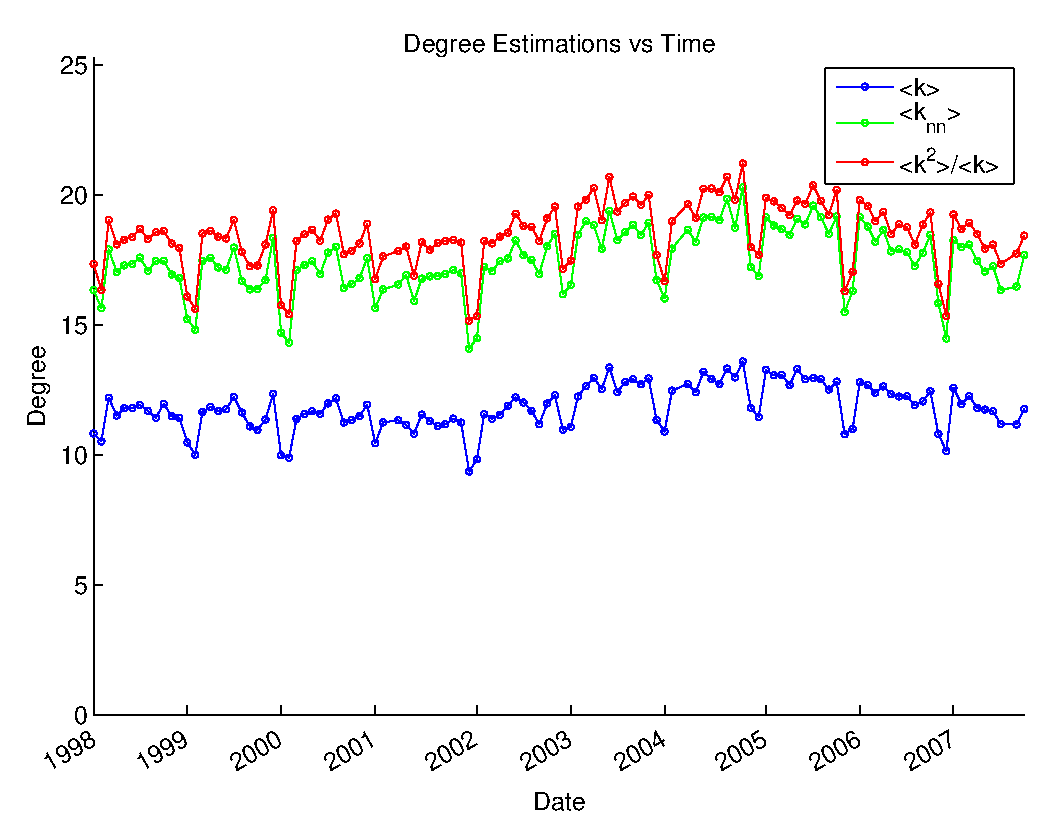
\includegraphics[width = .8\textwidth]{Graficos/NearestNeighbors.eps}
\caption{Changes in the average number of nearest-neighbor links (average grade of all of the nodes in the network) over time.}
\label{fig:NearestNeighbors}
\end{figure}

% \subsubsection*{Nearest neighbor calculations}
The degree of the node \(i\) in a given time step \(m\):
\begin{equation}
k_{i,m} = \sum_j a_{ij,m}
\end{equation}
The average degree of all nodes in the network, \emph{excluding} nodes that are not currently participating in the network, that is to say, excluding nodes with \(k_{i,m} = 0\).

\begin{equation}
<k>_m = \frac{1}{N_m}\sum_i k_{i,m} 
\end{equation}
Shown above is the evolution of \(<k>_m\) as \(m\) increases, or the average number of nearest neighbors of all the nodes in the network over time.

The metric \(R\) over time:
\begin{equation}
R_m = \frac{<k^2>_m}{<k>_m}
\end{equation}
Shown above is the evolution of \(R_m\) as \(m\) increases, or the value of \(R\) for each monthly graph varying over time. \(R\) is an estimation of \(k_{nn}\) for uncorrelated graphs, and since \(R \approx k_{nn}\) for this network, we can say that it is uncorrelated.

The average degree of the nearest neighbors of a node \(i\) in time step \(m\) is given by:
\begin{equation}
k_{{nn}_{i,m}} = \frac{1}{k_{i,m}} \sum_{j}  a_{ij,m}  k_{j,m}
\end{equation}

Then the average \(<k_{nn}>_m\) is graphed, to show how the average nearest-neighbor degree changes over time. Note that this average also excludes all nodes not participating in the network.
\begin{equation}
<k>_m = \frac{1}{\sum_j }\sum_i a_{ij,m} k_{{nn}_{i,m}}
\end{equation}

\begin{figure}[H]
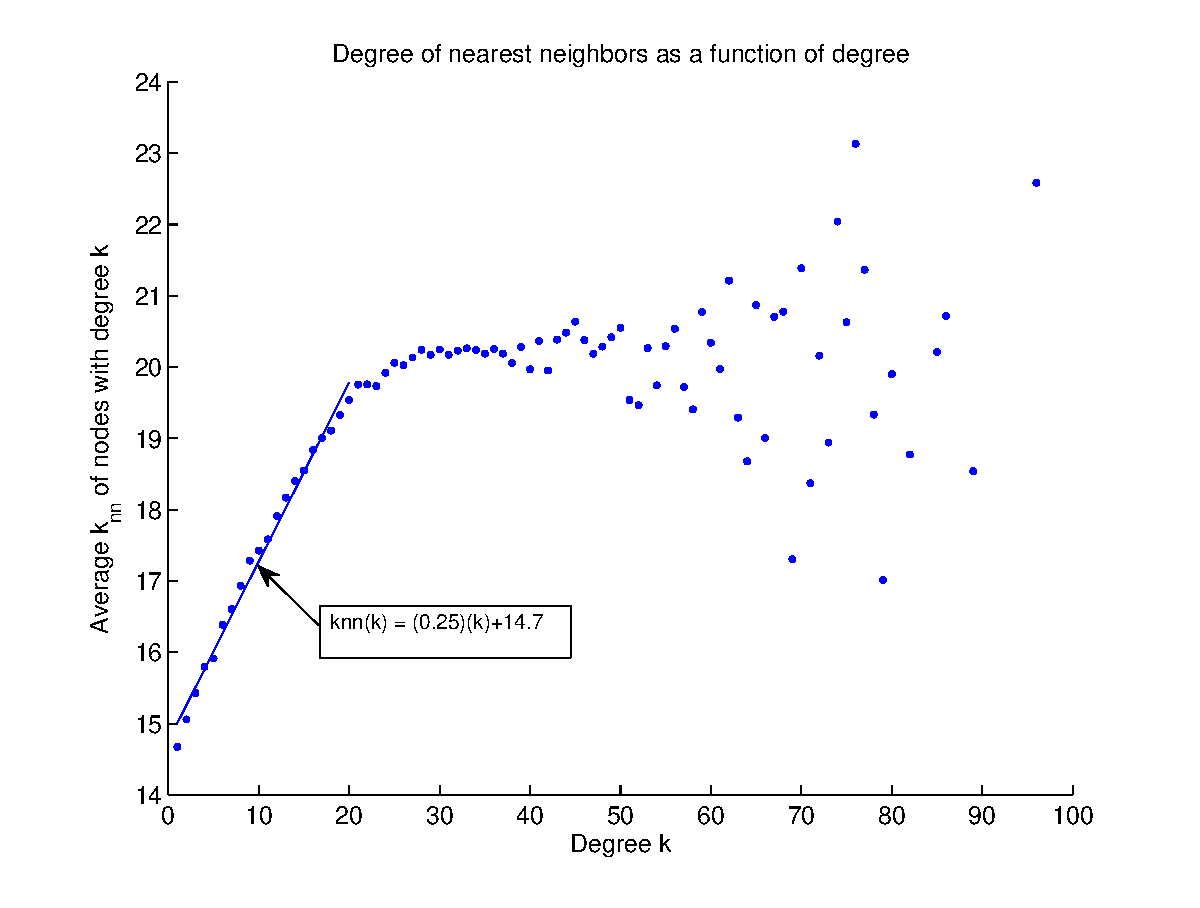
\includegraphics[width = 1\textwidth]{Graficos/knnvskA.eps}
\caption{For \( 1 \leq k \leq 20\) (\(88\%\) of the participating nodes in the network have \(k_i\) values in this range, the relationship between \(k\) and \(k_{nn}\) can be described by the given linear approximation, that \(k_{nn}(k) = 0.25k + 14.7\). As \(k\) becomes very large, however, this relationship plateaus, and for very large \(k\) there simply is not a large enough sample set of nodes to get a good average.}
\label{fig:knnvsk}
\end{figure}

\begin{figure}[H]
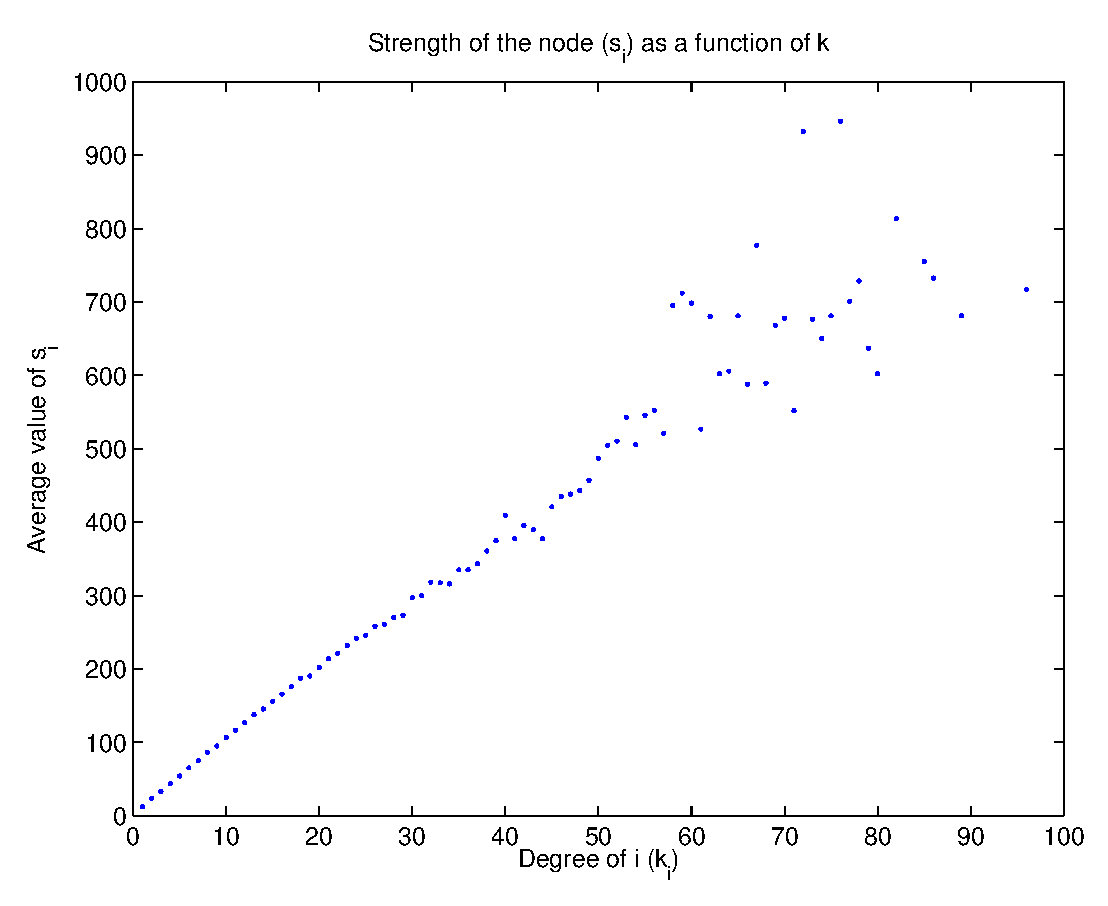
\includegraphics[width = 1\textwidth]{Graficos/svsk.eps}
\caption{Relationship between the strength of node \(i\) and the degree of node \(i\) (\(k_{i,m}\)). The relationship between \(\ln{(k_i)}\) and \(s_i\) appears to be roughly linear, which means that \(s_i \propto k_i^\alpha\). This relationship indicates that the more edges \(i\) has the more weight each edge has. In our case, the more other nodes \(i\) is connected to the more calls per relationship \(i\) makes. \newline A similar study on time-evolving social networks notes that: \newline ``This super-linear association between number of contacts and their average duration is the statistical signature of super connectors that not only develop a large number of distinct interactions, but also dedicate an increasingly larger amount of time to such interactions" [Cattuto].}
\label{fig:svsk}
\end{figure}

Strength node \(i\):
\begin{equation}
s_{i,m} = \sum_{j=1}^N w_{ij,m}
\end{equation}

\begin{figure}[H]
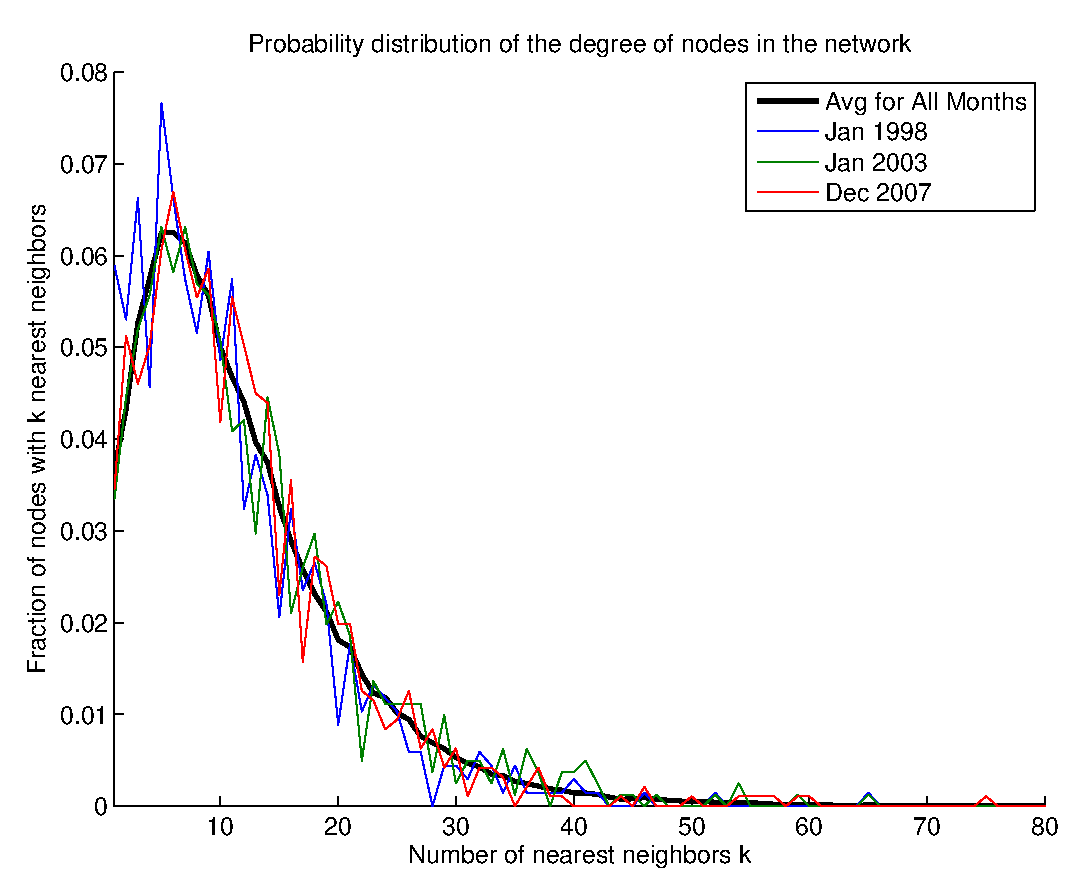
\includegraphics[width = .9\textwidth]{Graficos/ProbDistk.eps}
\caption{The probability distribution of the degrees of the nodes in the network, i.e., how probable it is that a certain node will have some degree. Note that only participating nodes (\(i \text{ s.t. } k_i \neq 0\)) are considered. \newline The mean value of \(k\), \(\mu_k\), such that \(P(k_i < \mu_k) = 0.50\) for the probability distribution \(P_k\) averaged over all time steps is \(\mu_k = 8.5\).
The distribution function does not change much in time. }
\label{fig:ProbDistk}
\end{figure}

Note that ``participating nodes" is determined per time step.
\begin{equation}
P_k = \frac{\text{number of nodes with degree \( k \)}}{\text{total participating nodes}}
\end{equation}

\subsubsection{Topological similarity in time}

From ``Graph Metrics for Temporal Networks" by Nicosia et al, we use the \emph{temporal correlation coefficient} (with one change to correct for the fact that not all of the nodes in our network are participating at any given time) to measure the topological overlap between social networks in different time steps.

\begin{equation}
C_i(t_m,t_{m+1}) = \frac{ \sum_j a_{ij}(t_m)a_{ij}(t_{m+1})}{\sqrt{[ \sum_j a_{ij}(t_m)][ \sum_j a_{ij}(t_{m+1})]}}
\label{eq:Ci}
\end{equation}

\begin{equation}
C_m = \frac{1}{\max [N_m,N_{m+1}]} \sum_{i = 1}^{N} C_i(t_m,t_{m+1})
\label{eq:Cm2}
\end{equation}

\begin{equation}
C = \frac{1}{M-1}\sum_{m=1}^{M-1}  C_m
\label{eq:C2}
\end{equation}

Note that \(0 < C < 1\), with \(C = 1\) if and only if the two graphs being compared are exactly alike and \(C =0 \) if and only if the graphs being compared have no edges in common.  Also note that while \(C\) represents the similarity between two graphs, it is not exactly the fraction of the graph that remains the same, so be careful when comparing \(C\) to other metrics, rather than comparing \(C\) values with each other.

\begin{table}[H]
\begin{tabular}{ |c|c|c|c| }
\hline
\multicolumn{4}{ |c| }{Temporal Correlation Coefficient} \\
\hline
10 year span & 5 year span & 2.5 year span & 1.25 year span \\ \hline
\multirow{8}{*}{0.5200}% {\parbox{1cm}{01/1998 --  12/2007}} 
 & \multirow{4}{*}{0.5359} & \multirow{2}{*}{0.5338} & 0.5297\\ \cline{4-4}
 &   &  & 0.5376 \\ \cline{3-4}
 &   &  \multirow{2}{*}{0.5380} & 0.5621 \\ \cline{4-4}
 &   &   & 0.5139\\ \cline{2-4}
 & \multirow{4}{*}{0.5037} &  \multirow{2}{*}{0.4994} & 0.4994\\ \cline{4-4}
 &   &   & 0.4994 \\ \cline{3-4}
 &   &  \multirow{2}{*}{0.5081} & 0.5103 \\ \cline{4-4}
 &   &   & 0.5056 \\ \hline
\end{tabular}
\caption{Shows the average topological overlap between time steps over varying time periods (for instance, the second column shows \(C\) for the first and second five-year periods in the observed time-window). The temporal correlation seems relatively uniform in time, that is, the first fifteen months are not significantly more or less correlated than the last fifteen months.}
\end{table}

\begin{figure}[H]
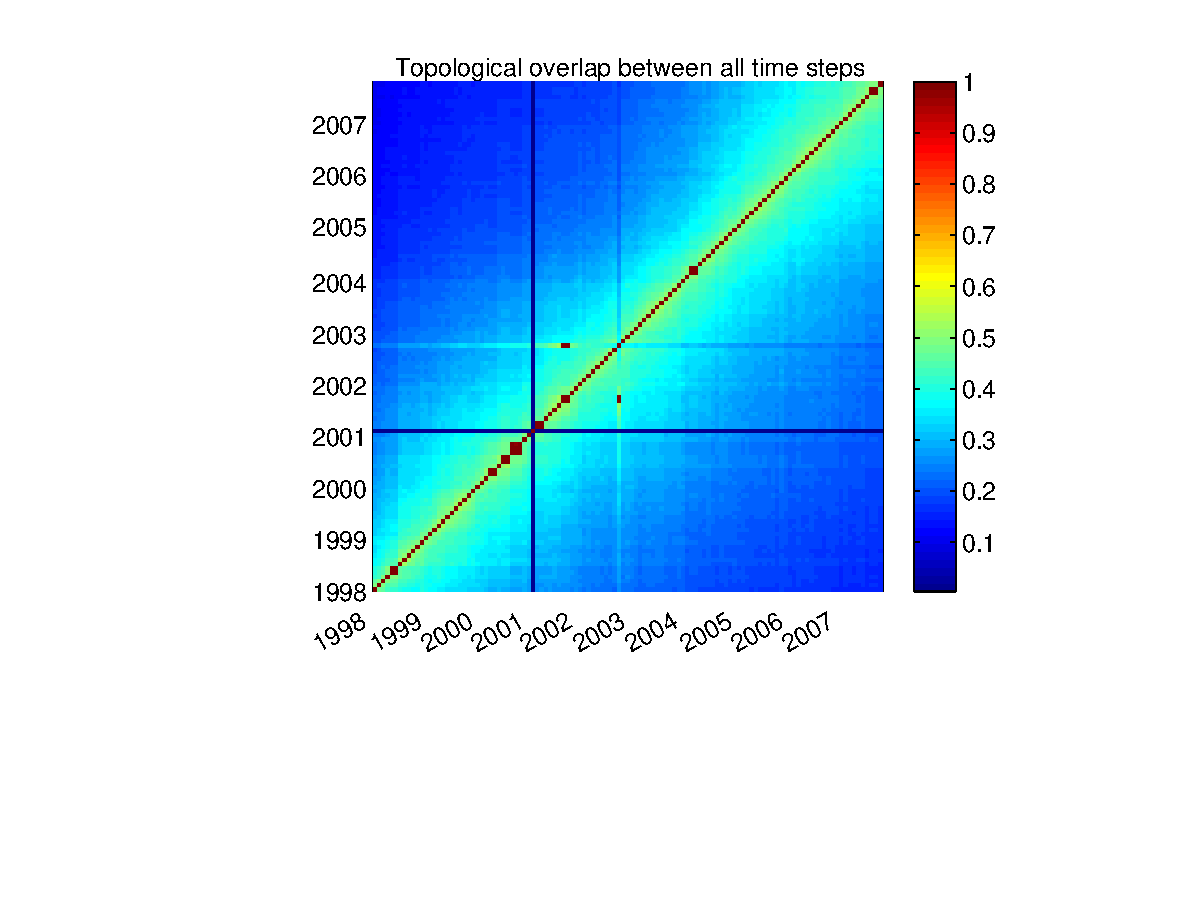
\includegraphics[trim=4.5cm 4cm 3.1cm 0.7cm, clip=true, width = .95\textwidth]{Graficos/overlap.eps}
\caption{Topological overlap between each month and every other month. Red along the diagonal corresponds to the comparison of each month to itself (\(C = 1\)), and, as expected, correlation decreases as the months being compared are farther apart in time. The anomaly mentioned in section 1.1.1 can be seen clearly here, with the dark blue lines for month 38.}
\label{fig:overlap}
\end{figure}

The average temporal correlation between some time step and any other time step is \(C = 0.2705\), which is the approximate value of \(C\) if the temporal correlation between graphs is removed entirely (that is, the sequencing of the time series is randomized). As expected, this is lower than the overlap between subsequent graphs, indicating that the network is changing significantly and permanently, rather than simply experiencing fluctuations.

\subsection{Internet adoption}

This project began with the assumption that once a user had adopted internet, they would rarely, if ever, give it up. However, the adoption data that we have shows something very different: many users adopt and then abandon internet use, and the median number of fluctuations for users (nodes who adopt at least once) is 2, meaning that most users abandon internet service (``recover") at least once, and more than a quarter of users fluctuate more than 4 times. Also, 282 nodes adopt internet at least once, while only 185 have internet service at the end of the observed time period in December 2007.

The prominence of a recovery class makes it clear that more thought needs to be devoted to distinguishing between first-time adopters and users transitioning to having internet from having no internet when computing these metrics.

\begin{figure}[H]
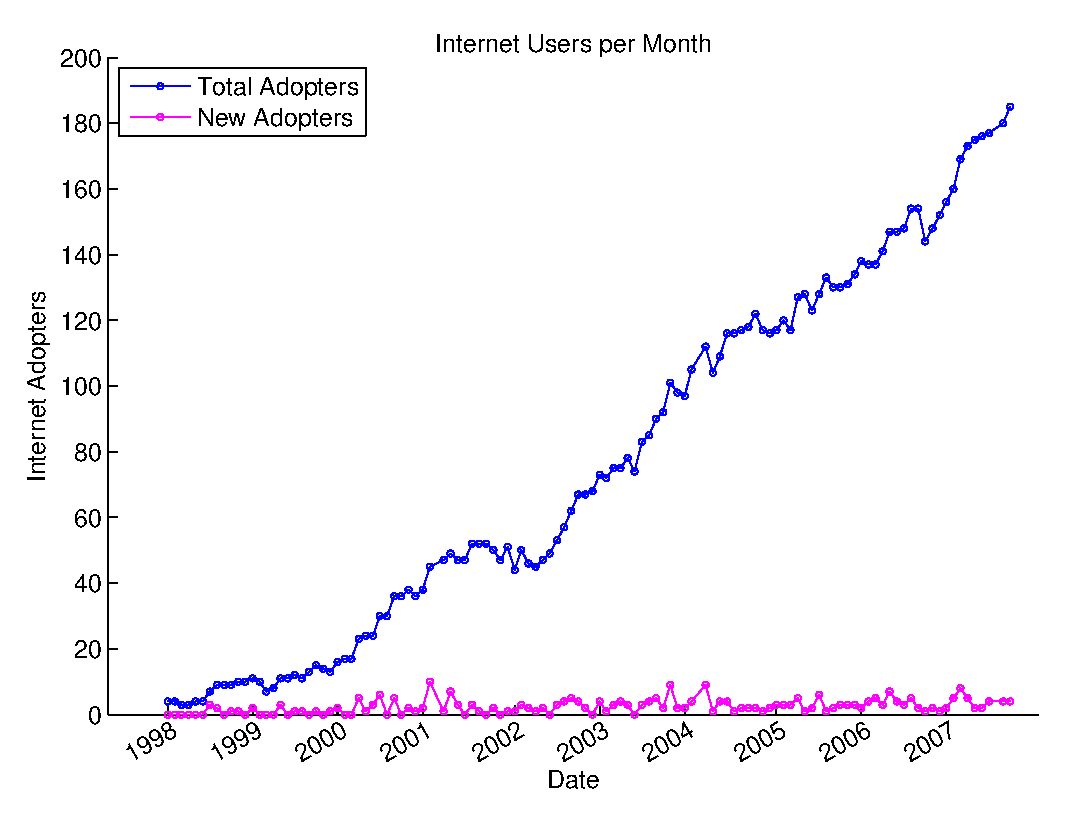
\includegraphics[width = .8\textwidth]{Graficos/AdoptersperMonth.eps}
\caption{Plot showing the number of adopters per month. Note that the number of new adopters per month does not change greatly and the number of total adopters grows linearly.}
\label{fig:AdoptersperMonth}
\end{figure}

\begin{figure}[H]
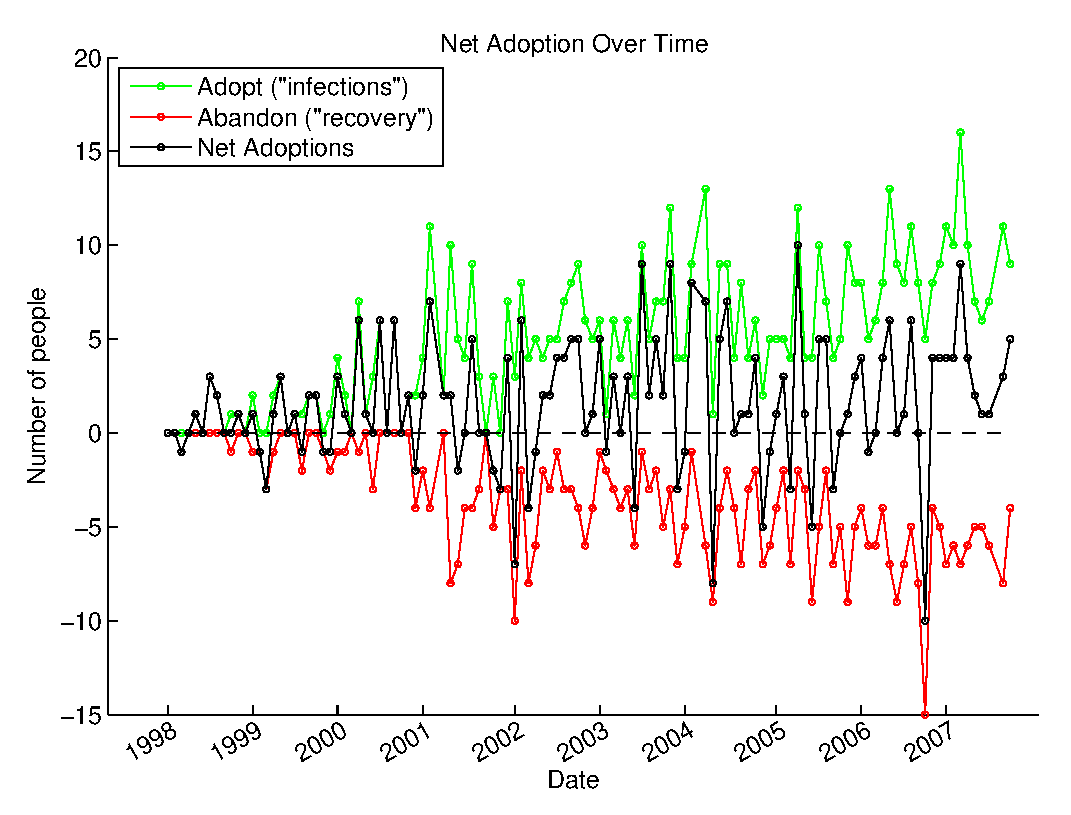
\includegraphics[width = .8\textwidth]{Graficos/trans.eps}
\caption{Fluctuations per month. Green shows the number of people who transition from susceptible to infected (S \(\rightarrow\) I), red the number of people who transition from infected to recovered (I \(\rightarrow\) R), and black the net change in the total number of adoptions for the given month.}
\label{fig:trans}
\end{figure}

%\begin{figure}[H]
%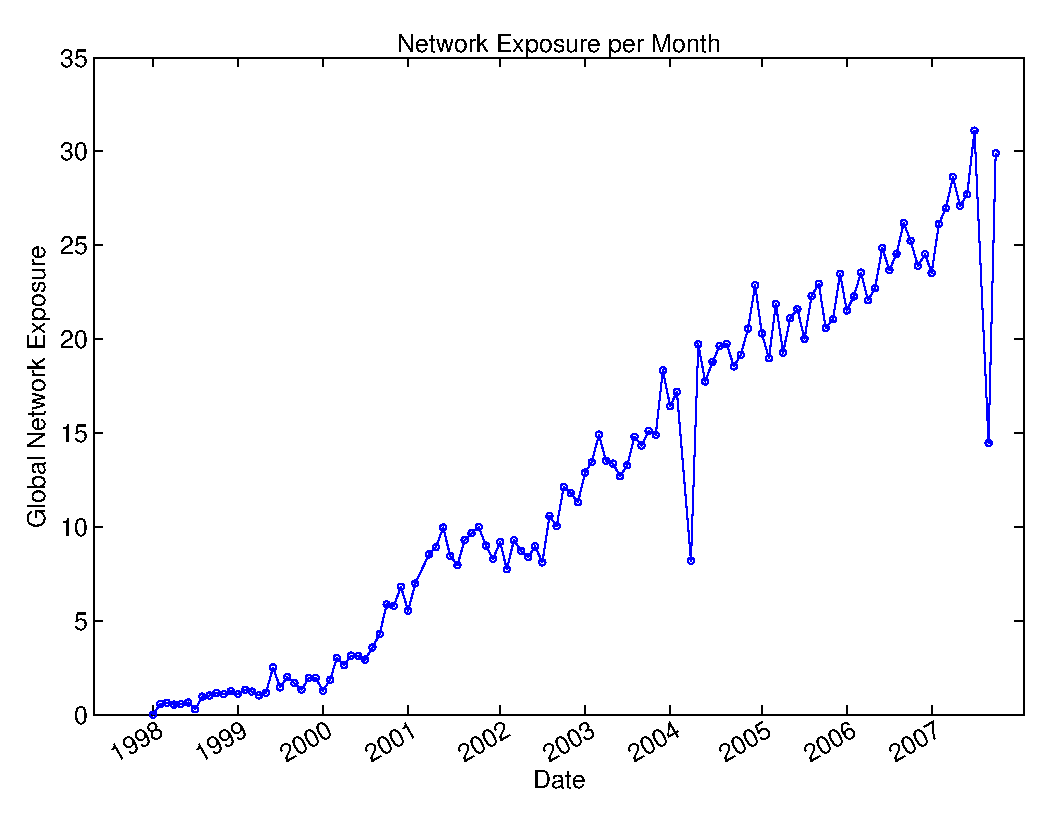
\includegraphics[width = .9\textwidth]{Graficos/GNEperMonth.eps}
%\caption{GNEperMonth}
%\label{fig:GNEperMonth}
%\end{figure}
%
%\begin{figure}[H]
%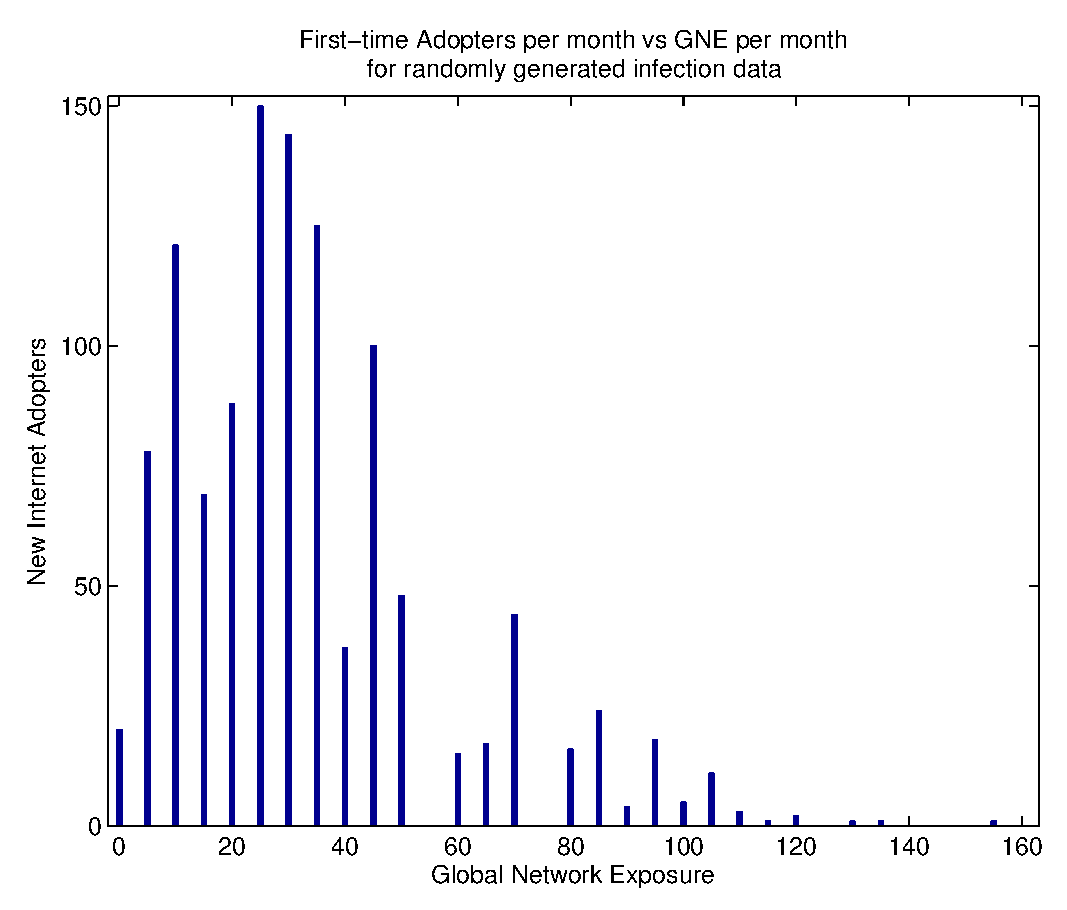
\includegraphics[width = .9\textwidth]{Graficos/GNEvsNewAdopters.eps}
%\caption{GNEvsNewAdopters}
%\label{fig:GNEvsNewAdopters}
%\end{figure}

%\begin{figure}[H]
%\includegraphics[width=\textwidth]{Graficos/AdoptionsvsGNE.eps}
%\caption{AdoptionsvsGNE}
%\label{fig:AdoptionsvsGNE}
%\end{figure}

%\begin{figure}[H]
%\includegraphics[width=\textwidth]{Graficos/RandomInfection/PreserveMonthlyTotals/AdoptionsvsGNE.eps}
%\caption{AdoptionsvsGNErand. preserve monthly totals in Adoption}
%\label{fig:AdoptionsvsGNErand}
%\end{figure}
%
%\begin{figure}[H]
%\includegraphics[width=\textwidth]{Graficos/GNEvsk.eps}
%\caption{GNEvsk}
%\label{fig:GNEvsk}
%\end{figure}
%
%\begin{figure}[H]
%\includegraphics[width = .9\textwidth]{Graficos/RandomInfection/PreserveMonthlyTotals/GNEvsk.eps}
%\caption{GNEvskrand}
%\label{fig:GNEvskrand}
%\end{figure}
%
%THINGS
%
%\begin{figure}[H]
%\includegraphics[width=\textwidth]{Graficos/AdoptionsPerk.eps}
%\caption{AdoptionsPerk. The "COM" of the data is at about 15.5. Note that \(<k>= 8.6, <k>\) without non-participants  = 11.9}
%\label{fig:AdoptionsPErk}
%\end{figure}
%
%\begin{figure}[H]
%\includegraphics[width = .9\textwidth]{Graficos/RandomInfection/PreserveMonthlyTotals/AdoptionsPerk.eps}
%\caption{AdoptionsPerkRand. The "COM" of the data is at about 9.25}
%\label{fig:AdoptionsPerkRand}
%\end{figure}

%\begin{figure}[H]
%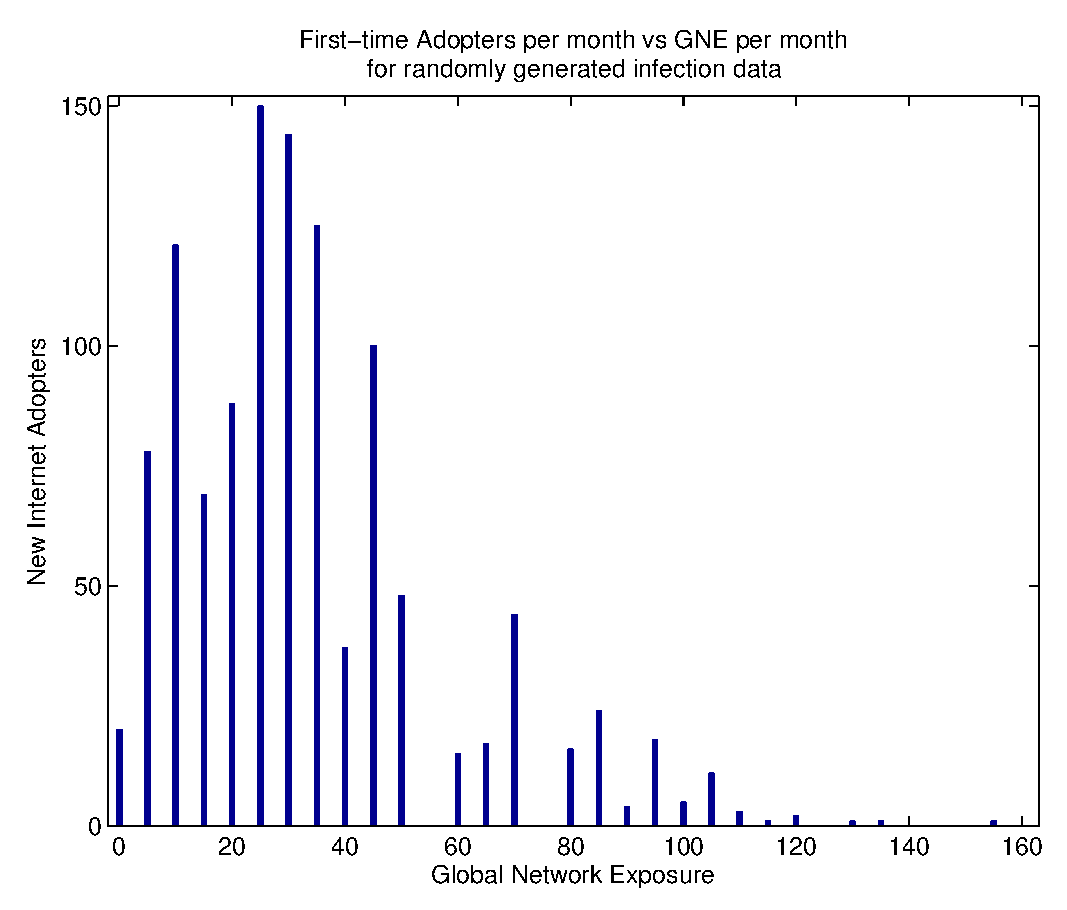
\includegraphics[width = .9\textwidth]{Graficos/GNEvsNewAdopters.eps}
%\caption{GNEvsNewAdopters}
%\label{fig:GNEvsNewAdopters}
%\end{figure}

\subsection{Measuring contagion}

One metric that we are experimenting with to measure contagion is PNE, or \emph{personal network exposure}. Note that PNE is calculated in the same way for both adopters and non-adopters (as opposed to other sources which have noted PNE as applying only to not-yet adopters).

\begin{equation}
{\it PNE}_{{i}} \left( n \right) ={\frac {\sum _{j=1}^{k_{{i}}}
 W_{{i,j}} \left( n \right) Y_{{j}} \left( n-1
 \right) }{\sum _{j=1}^{k_{{i}}}  W_{{i,j}} \left( n
 \right) }}
 \label{eq:PNE}
\end{equation}

Then GNE, or \emph{global network exposure} is simply the sum of the personal network exposure for all nodes for a given month.
 
\begin{equation}
{\it NE} \left( n \right) =\sum _{i=1}^{N}{\it PNE}_{{i}} \left( n
 \right) 
\end{equation}

%\begin{figure}[H]
%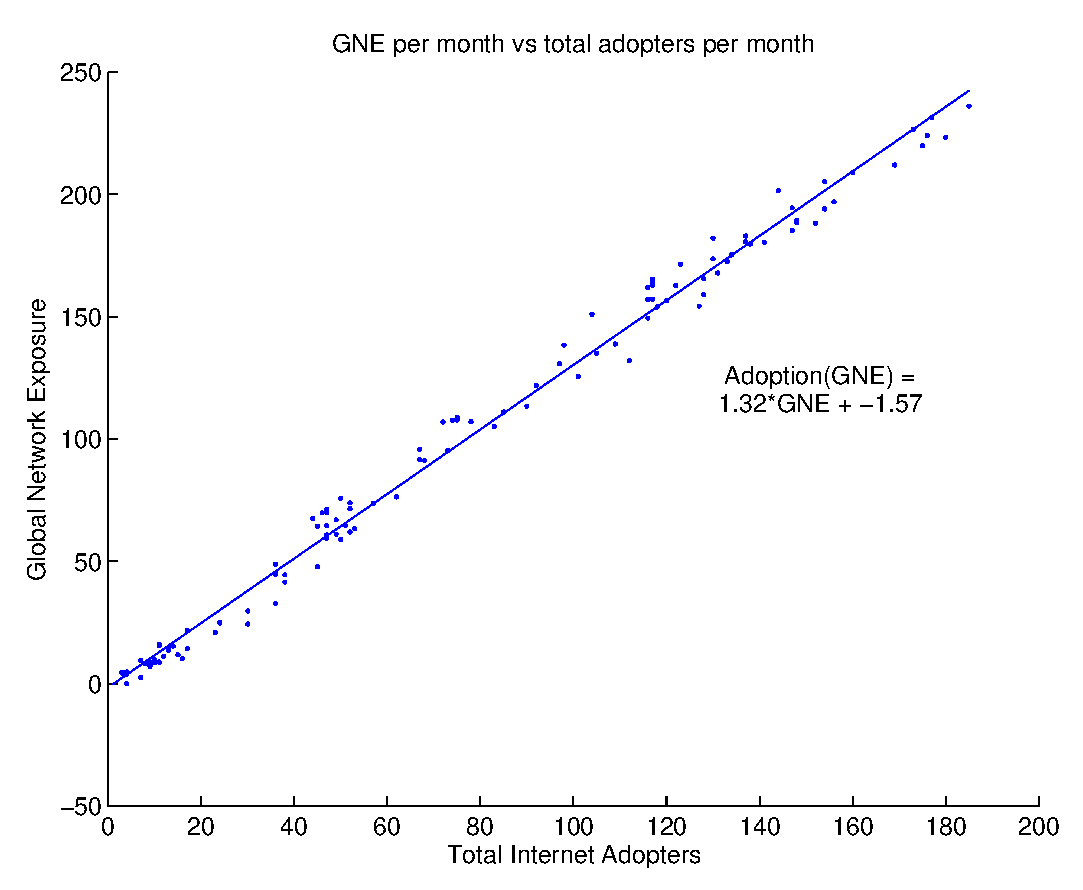
\includegraphics[width = .9\textwidth]{Graficos/GNEvsTotalAdopters.eps}
%\caption{GNEvsTotalAdopters. A larger GNE, in general, means more adopters. }
%\label{fig:GNEvsTotalAdopters}
%\end{figure}

%\begin{figure}[H]
%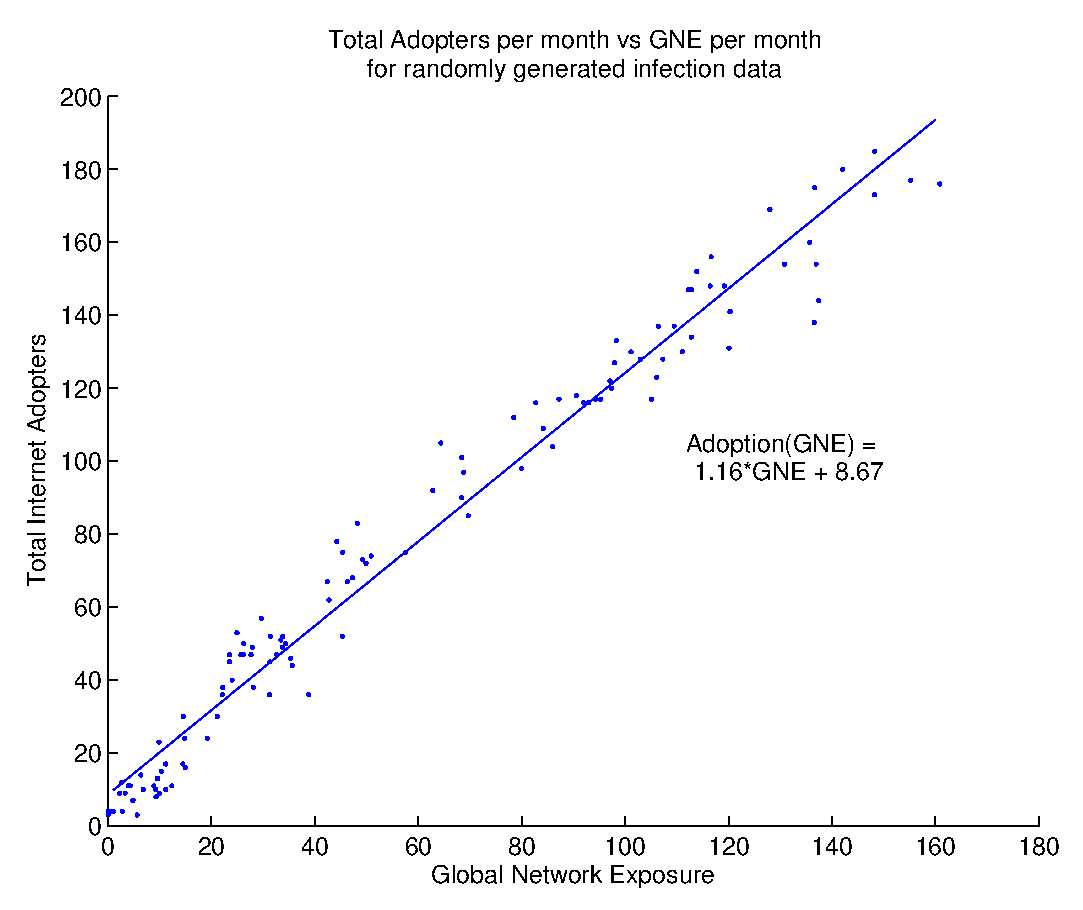
\includegraphics[width = .9\textwidth]{Graficos/RandomInfection/GNEvsTotalAdopters.eps}
%\caption{Random infection data was generated by randomly reassigning adoption attributes of nodes, while preserving the total number of ``infected" nodes per time step. There still exists a tight correlation between the number of adopters and the GNE, but the GNE is substantially lower.}
%\label{fig:GNEvsTotalAdoptersRand}
%\end{figure}
%
%Dependance of the GNE on the topology of the network as well as the number of adopters indicates that GNE could be a viable metric for indicating ``contagion," or at least the connectedness of adopters and non adopters.

\begin{figure}[H]
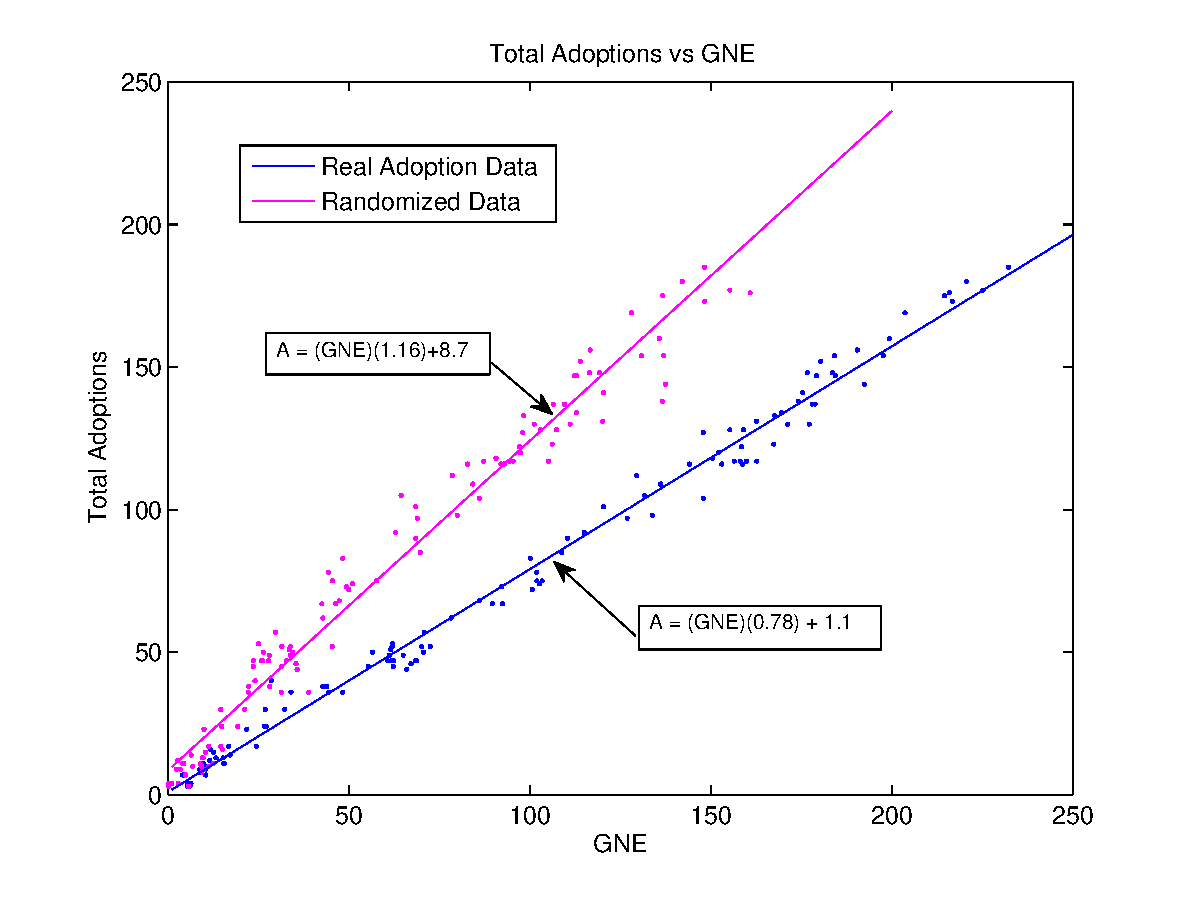
\includegraphics[width = .9\textwidth]{Graficos/GNEandGNErandom2.eps}
\caption{Compares the correlation between the global network exposure (GNE) and adoption for the real data set and for a data set that was randomly generated by randomly reassigning the attribute of adoption to nodes in the network, preserving the number of adoptions per month but destroying the correlation between the network and adoption.}
\label{fig:GNEandGNErandom}
\end{figure}

\begin{figure}[H]
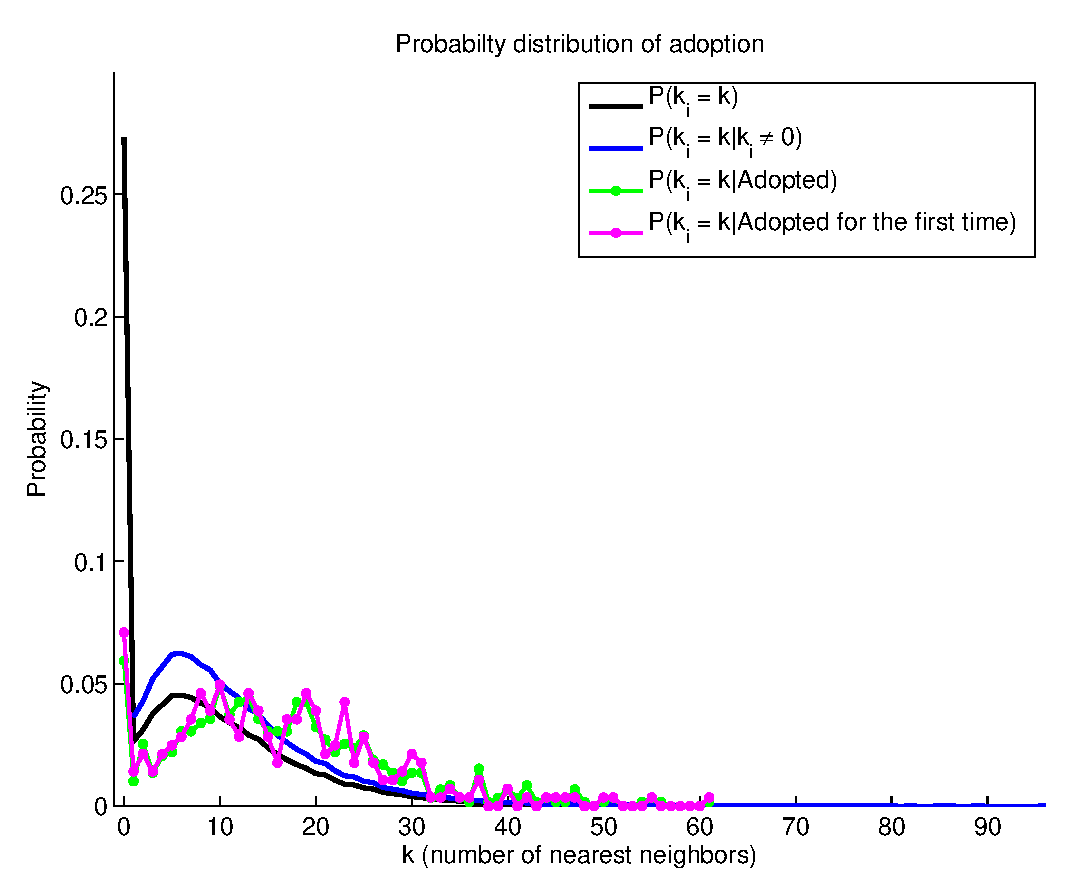
\includegraphics[width = .9\textwidth]{Graficos/PkGivenAdopt.eps}
\caption{PkGivenAdopt.eps. \newline For all adopters: \(P(k_i =k | S \rightarrow I),P(k_i < 15.2 | S \rightarrow I) =0.50\) \newline For first time adopters: \(P(k_i =k | S \rightarrow I), P(k_i < 14.5 | S \rightarrow I) =0.50\) 
\newline That is to say, for a group of adopters, the mean degree is significantly higher than the mean grade of the general population.}
\label{fig:PkGivenAdopt}
\end{figure}

\begin{figure}[H]
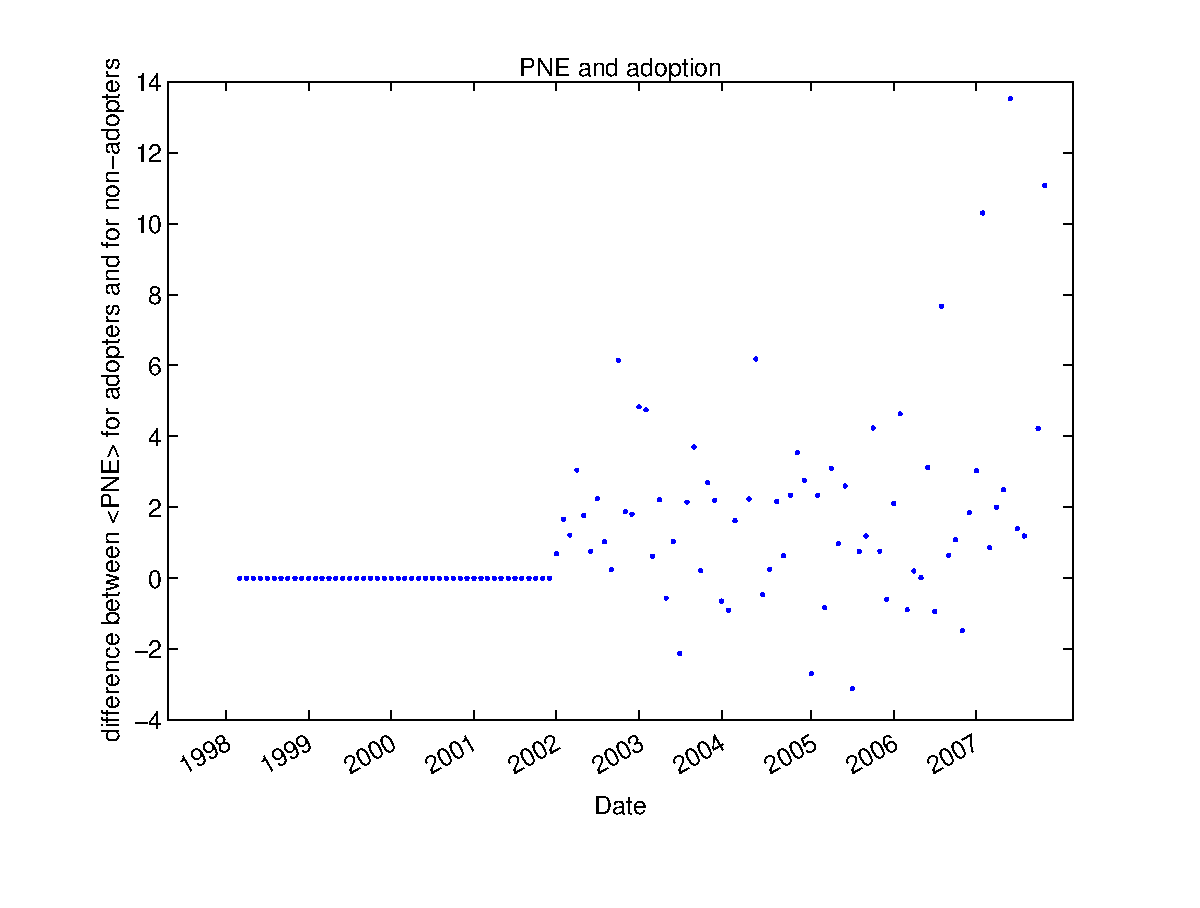
\includegraphics[width = \textwidth]{Graficos/PNEandAdoption.eps}
\caption{This graph is looking at the connection between PNE and adoption; each point is calculated as shown below.}
\label{fig:PNEandAdoption}
\end{figure}

The total network exposure of the adopting node \(i\):
\begin{equation}
E_{i,m} = \sum_1^m PNE_{i,m}
\label{eq:PNEandAdopt}
\end{equation}

Then the difference between \(<E>_m\) for adopting nodes and \(<E>_m\) for the general population of nodes in each time step is plotted. That is, ever positive point on the plot shows a time set where adopters, on average, had higher network exposure than the general population. We can see that while the time series generally positive, it is not necessarily positive, and at the beginning of the period the adoption rate is so low that PNE is zero for both adopters and non-adopters.

\section{Conclusions}
Looking at traditional graph metrics, such as degree and nearest neighbor degree, we were able to conclude that the topology of the graph does not change much over time, and values such as \(<k>, <k^2> \text{ and } R\) can be treated as constant values. Over all of the time steps, the graphs appear uncorrelated.

Adoption data showed an unexpected prominence of recovery from \(I \rightarrow R\), (adopter to non-adopter) which was unexpected. When adoption data is combined with data about the network, it is important to consider carefully the difference between an adopter and a first-time adopter.

First attempts at demonstrating contagion lie in characterizing the topological differences between adopter nodes and non-adopter nodes. We also demonstrate the dependance of the metric GNE on both total adoption and the nodes which adopt.

\section{Future Work}
To continue, first the anomalies discussed in section 1 need to be addressed. From there moving forward, we are looking to further examine the role of weights in the network, evaluate clustering coefficients for the network, and continue to test the metrics that we are using by doing comparisons with randomized network data (to justify that the correlations we see are functions of the network, not simply inherent in the metrics used).



%\begin{figure}[H]
%\includegraphics[width = .9\textwidth]{Graficos/PkGivenFirstAdopt.eps}
%\caption{PkGivenFirstAdopt.eps \(P(k_i =k | S \rightarrow I), \mu_k = 14.5\). }
%\label{fig:PkGivenFirstAdopt}
%\end{figure}


\end{document}
